% Section 6 : Performances (partie factuelle)
% Chaque chiffre : resultats/chiffres_rapport.md (bloc de lignes du CSV),
% resultats/scenarios.md ou resultats/exemples_rapport.md.
% Temps : moyenne ± écart-type ; états : sans l'état puits.

\section{Performances}
\label{sec:performances}

\subsection{Protocole}

Toutes les mesures ont été faites sur la même machine : un Intel Core
i5-8350U (4 cœurs, 8 threads, 1,7~GHz) avec 7,6~Go de mémoire, sous
Ubuntu 24.04 (Linux 6.17), avec OpenJDK 21 (notre code est compilé en
bytecode Java 11) et GNU \texttt{grep} 3.11.

Nous mesurons de deux façons. \emph{En mémoire} (\texttt{bench/Benchmark.java}) :
le texte est chargé une seule fois, puis chaque cas fait 5 tours de
chauffe et 20 mesures avec \texttt{System.nanoTime}. On chronomètre à part
la construction (analyse de la regex, automate ou fonction d'échec $\pi$)
et la recherche. \emph{De bout en bout} (\texttt{bench/bench\_bout\_en\_bout.py}) :
on chronomètre 10 lancements complets de \texttt{java -jar} et de
\texttt{grep -E -c}, démarrage compris. Chaque configuration tourne dans
sa propre JVM. Dans une JVM commune, le compilateur JIT optimisait le
code partagé (\texttt{AfdCompile.suivant}) pour l'algorithme mesuré en
premier, et le suivant paraissait plus lent qu'il ne l'est : l'ordre des
mesures changeait le résultat. Nous donnons la moyenne $\pm$ l'écart-type,
et aussi la médiane quand l'écart-type est grand.

\subsection{Le lecteur : chercher un nom dans un livre}

On cherche les lignes où apparaît un personnage : le motif est un mot
sans opérateur.
\begin{verbatim}
F=data/tour-du-monde-800.txt
java -jar egrep-clone.jar --stats -c Passepartout $F
\end{verbatim}
Notre programme reconnaît un littéral et choisit KMP : pas d'AFN-$\varepsilon$,
pas de construction des sous-ensembles, seulement la fonction d'échec
$\pi$. Il trouve 423 lignes, comme \texttt{grep}.

Sur \emph{Don Quixote} en mémoire (figure~\ref{fig:kmp}), les 8
littéraux donnent :
\begin{itemize}
\item recherche avec KMP : de 3,305~$\pm$~0,039~ms (\texttt{III})
  à 5,752~$\pm$~0,106~ms (littéral de 70 caractères) ;
\item recherche avec l'automate et le matcher une passe :
  de 7,147~$\pm$~0,361~ms (\texttt{t’s n})
  à 9,489~$\pm$~1,622~ms (\texttt{ire of m}).
\end{itemize}
L'écart est surtout dans la construction. Pour le littéral de
70 caractères, la fonction d'échec prend 0,032~$\pm$~0,009~ms et
l'automate 10,490~$\pm$~1,969~ms. Cet automate est gros :
AFN-$\varepsilon$ de R : 140 états ; AFD minimal de \texttt{.*R} :
71 états. Sur 32~Mio, \texttt{together} prend 79,6~$\pm$~5,3~ms avec
KMP et 104,7~$\pm$~1,0~ms avec le matcher une passe.

\begin{figure}[htbp]
\centering
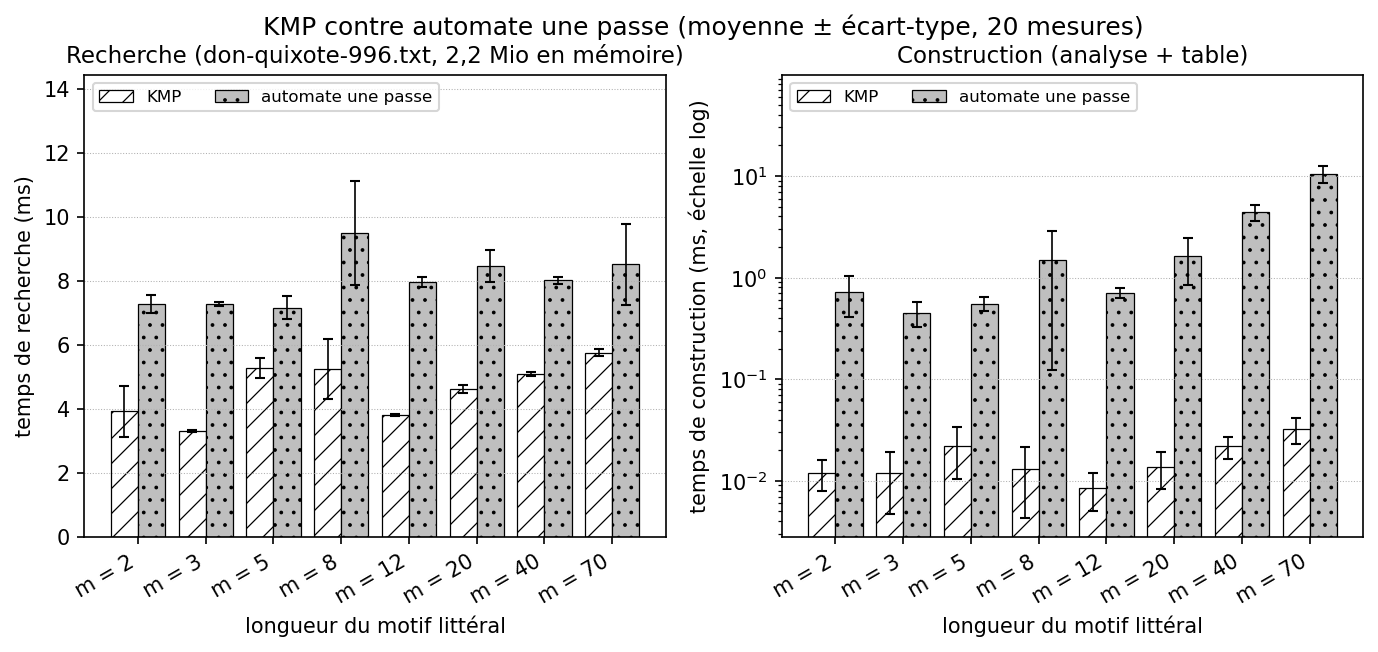
\includegraphics[width=0.8\linewidth]{figures/fig_kmp_vs_automate.png}
\caption{KMP contre automate (matcher une passe), 8 littéraux de 2 à 70
caractères sur \emph{Don Quixote} en mémoire : recherche à gauche,
construction à droite (échelle log).}
\label{fig:kmp}
\end{figure}

\subsection{Le chercheur et l'archiviste : une expression courante}

Le chercheur veut toutes les variantes d'un nom dans un livre ;
l'archiviste lance la même recherche sur un corpus de plusieurs mégaoctets.
\begin{verbatim}
java -jar egrep-clone.jar -c 'S(a|g|r)*on' data/babylon-56667.txt
\end{verbatim}
La regex n'est pas littérale : on construit l'automate, et le matcher une
passe est le choix par défaut. Pour \texttt{S(a|g|r)*on}, les AFD minimaux
de R et de \texttt{.*R} ont tous deux 4 états.

Sur les vrais textes (figure~\ref{fig:naif}), le matcher naïf gagne
souvent, malgré son pire cas en $O(n^2)$ : \texttt{S(a|g|r)*on} sur
\emph{Don Quixote} prend 4,510~$\pm$~0,242~ms avec le naïf et
7,147~$\pm$~0,029~ms avec le matcher une passe. Comme l'état puits est
retiré, chaque essai du naïf s'arrête dès le premier caractère qui n'est
pas un \texttt{S}. Le naïf perd quand le point fait durer les essais :
\texttt{.(Bab|Ass)y} sur \emph{Don Quixote} prend 9,345~$\pm$~2,004~ms
contre 7,188~$\pm$~0,176~ms.

Pour l'archiviste (figure~\ref{fig:echelle}), le temps croît linéairement
avec la taille. De 1 à 32~Mio, \texttt{S(a|g|r)*on} passe de
2,029~$\pm$~0,328 à 68,027~$\pm$~4,758~ms avec le naïf ($\times$\,33,5),
et de 3,695~$\pm$~0,296 à 104,871~$\pm$~0,675~ms avec le matcher une passe
($\times$\,28,4).

\begin{figure}[htbp]
\centering
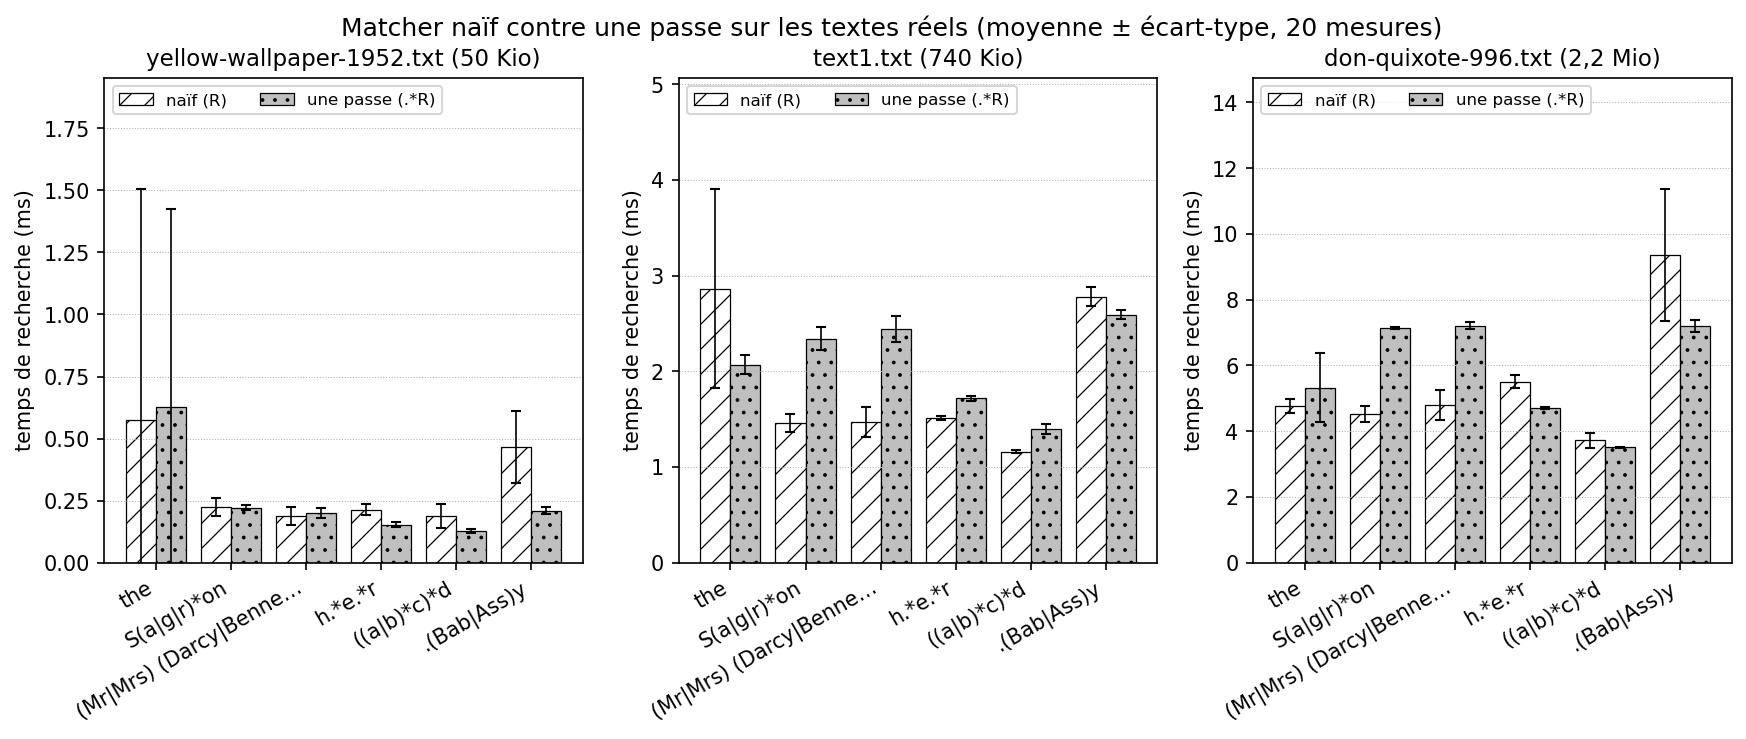
\includegraphics[width=\linewidth]{figures/fig_naif_vs_unepasse_textes.png}
\caption{Matcher naïf (automate de R) contre matcher une passe (automate
de \texttt{.*R}), 6 regex sur 3 textes réels, en mémoire.}
\label{fig:naif}
\end{figure}

\begin{figure}[htbp]
\centering
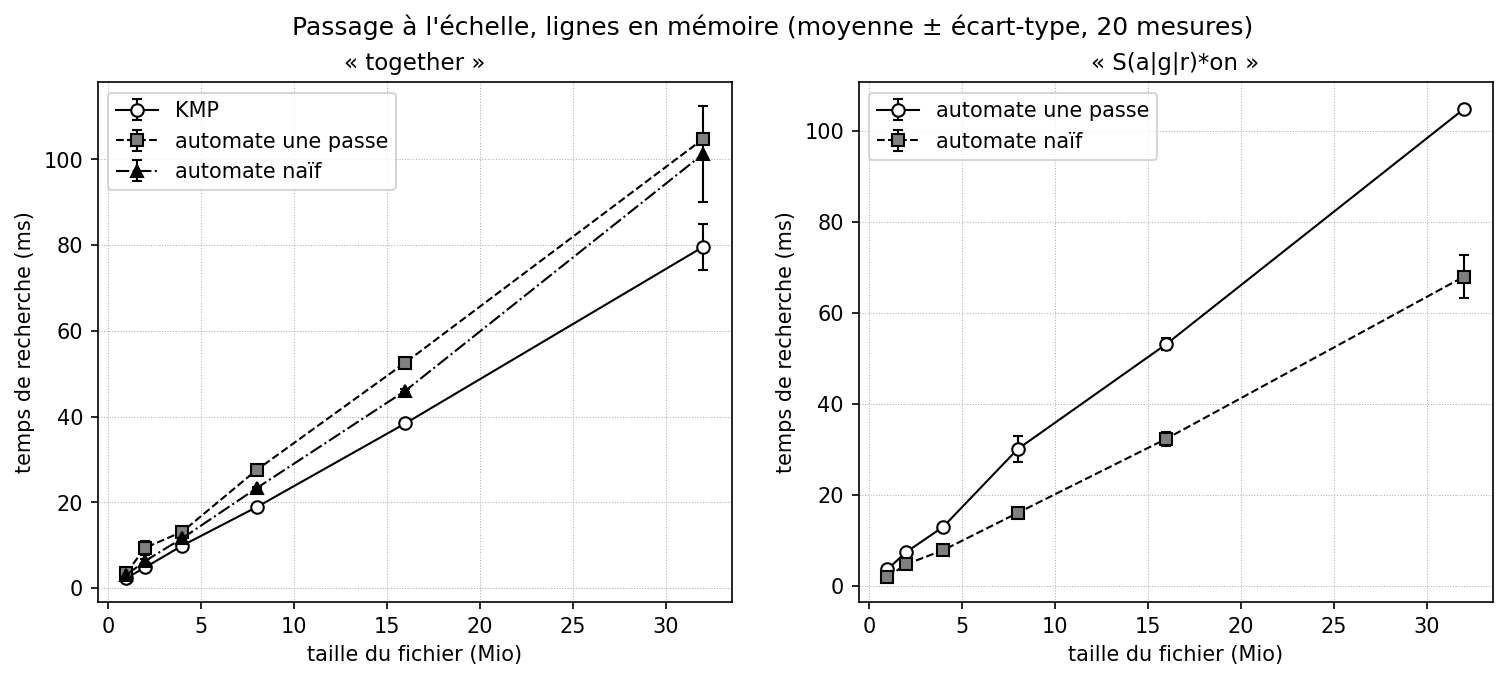
\includegraphics[width=0.75\linewidth]{figures/fig_passage_echelle.png}
\caption{Passage à l'échelle, fichiers de 1 à 32~Mio en mémoire :
\texttt{together} (KMP, naïf, une passe) et \texttt{S(a|g|r)*on} (naïf,
une passe).}
\label{fig:echelle}
\end{figure}

\subsection{Le piège : un livre sur une seule ligne}

Un texte a perdu ses retours à la ligne : ici, \emph{The Yellow Wallpaper}
recollé en une ligne de 50\,833 caractères.
\begin{verbatim}
tr '\n' ' ' < data/yellow-wallpaper-1952.txt > /tmp/une_ligne.txt
java -jar egrep-clone.jar --algo=automate --matcher=naif \
    -c 'e.*zq' /tmp/une_ligne.txt
\end{verbatim}
Le matcher une passe (le défaut) est le bon choix. Le matcher naïf relance
l'automate depuis chaque \texttt{e}, et \texttt{.*} lui fait lire toute la
fin de la ligne sans jamais trouver \texttt{zq}.

Sur la ligne unique (figure~\ref{fig:piege}, à gauche), \texttt{e.*zq}
prend 362,498~$\pm$~1,794~ms avec le naïf et 0,161~$\pm$~0,003~ms avec le
matcher une passe, soit 2\,249 fois moins. Sur le même livre en 1\,227
lignes, les deux restent sous la milliseconde (médianes 0,646~ms et
0,218~ms ; écarts-types grands, car c'est la première mesure de chaque JVM).
Sans \texttt{.*}, \texttt{S(a|g|r)*on} sur la ligne unique prend
0,162~$\pm$~0,009~ms et 0,161~$\pm$~0,003~ms : le découpage ne compte plus.
Le pire cas \texttt{a.*b} sur une ligne de $n$ lettres \texttt{a}
(figure~\ref{fig:piege}, à droite) montre la même chose. Entre $n = 10\,000$
et $n = 50\,000$, le naïf passe de 140,360~$\pm$~0,753 à
3\,547,938~$\pm$~39,825~ms (pente 2,01 en échelle log-log), et le matcher
une passe de 0,0348~$\pm$~0,0033 à 0,1632~$\pm$~0,0047~ms (pente 0,96).

Le coût du matcher une passe par caractère lu ne dépend presque pas du
cas (tableau~\ref{tab:ns}) : de 3,1 à 3,5~ns.

\begin{table}[htbp]
\centering
\small
\begin{tabular}{|l|l|r|r|r|}
\hline
Regex & Texte & Caractères & Temps (ms) & ns/car. \\
\hline
\texttt{a.*b} & ligne de 10\,000 \texttt{a} & 10\,000 & 0,0348~$\pm$~0,0033 & 3,5 \\
\texttt{a.*b} & ligne de 50\,000 \texttt{a} & 50\,000 & 0,1632~$\pm$~0,0047 & 3,3 \\
\texttt{e.*zq} & \emph{Yellow Wallpaper}, une ligne & 50\,833 & 0,1612~$\pm$~0,0033 & 3,2 \\
\texttt{S(a|g|r)*on} & \emph{Don Quixote} & 2\,275\,296 & 7,1471~$\pm$~0,0294 & 3,1 \\
\texttt{S(a|g|r)*on} & fichier de 32~Mio & 32\,429\,599 & 104,8706~$\pm$~0,6745 & 3,2 \\
\texttt{together} & fichier de 32~Mio & 32\,429\,599 & 104,7479~$\pm$~0,9794 & 3,2 \\
\hline
\end{tabular}
\caption{Coût du matcher une passe par caractère lu (lignes sans leur fin
de ligne). Seule une ligne de 1\,000 \texttt{a} sort du lot (6,7~ns) : la
mesure ne dure que 7~$\mu$s.}
\label{tab:ns}
\end{table}

\begin{figure}[htbp]
\centering
\begin{minipage}{0.49\linewidth}
\centering
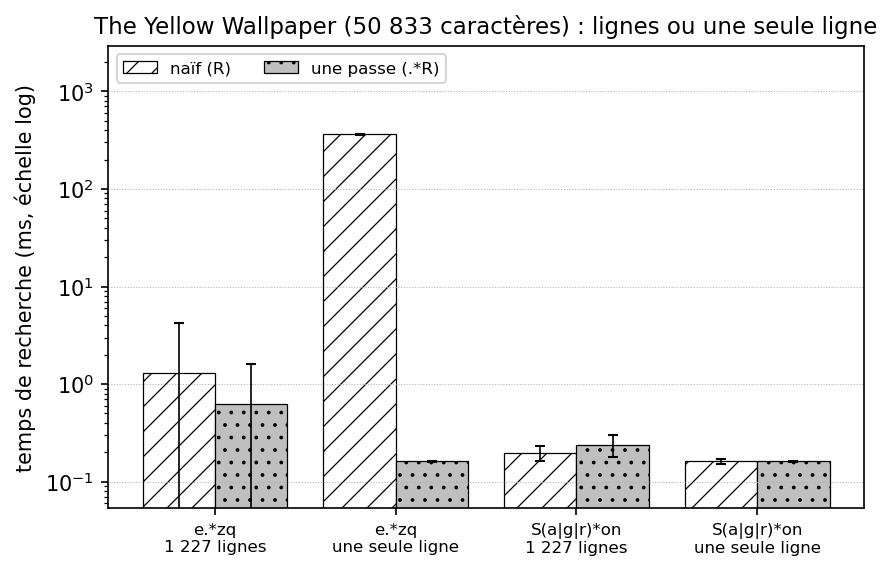
\includegraphics[width=\linewidth]{figures/fig_une_ligne.png}
\end{minipage}\hfill
\begin{minipage}{0.49\linewidth}
\centering
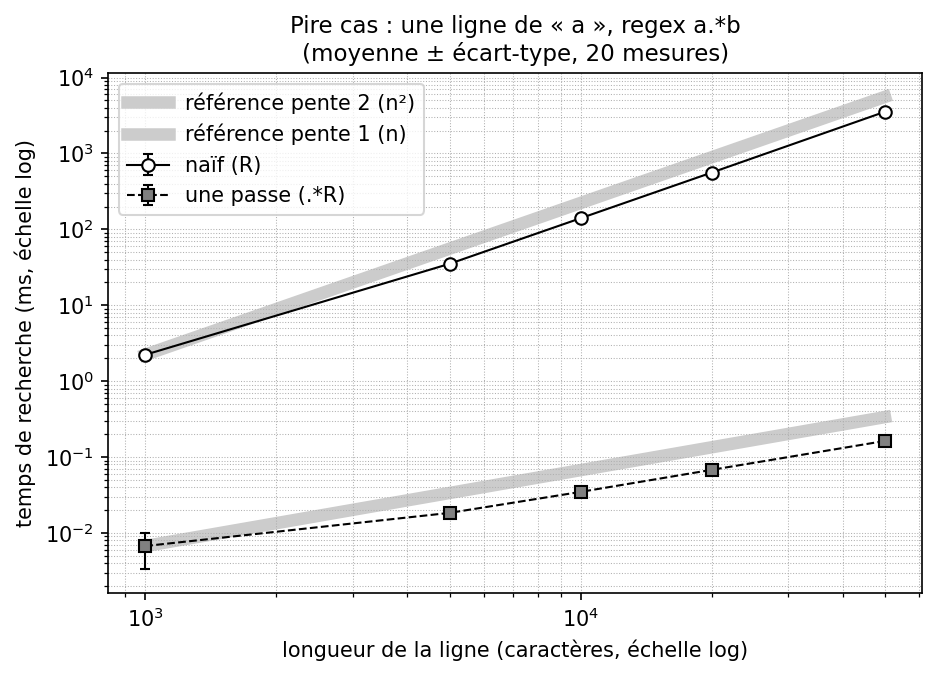
\includegraphics[width=\linewidth]{figures/fig_pire_cas.png}
\end{minipage}
\caption{À gauche : \emph{The Yellow Wallpaper} en 1\,227 lignes ou en une
seule ligne (échelle log). À droite : pire cas \texttt{a.*b} sur une ligne
de $n$ lettres \texttt{a}, avec les pentes 2 et 1 en référence.}
\label{fig:piege}
\end{figure}

\subsection{Le motif monstre : l'explosion des états}

Un motif court peut donner un automate énorme : \texttt{(a|b)*a}
suivi de $n$ fois \texttt{(a|b)}, c'est-à-dire un \texttt{a} suivi de
$n$ lettres \texttt{a} ou \texttt{b} (ici $n = 8$).
\begin{verbatim}
echo abaaaaaaaa | java -jar egrep-clone.jar --stats \
    '(a|b)*a(a|b)(a|b)(a|b)(a|b)(a|b)(a|b)(a|b)(a|b)'
\end{verbatim}
KMP ne s'applique pas : c'est l'automate. La construction des sous-ensembles
doit retenir quelles lettres, parmi les $n+1$ dernières, sont des
\texttt{a}, et la minimisation ne peut rien fusionner.

L'AFN-$\varepsilon$ grandit de 6 états par $(a|b)$ (16 états pour $n = 1$,
58 pour $n = 8$), mais l'AFD minimal a exactement $2^{n+1}$ états : 4 pour
$n = 1$, 512 pour $n = 8$, pour R comme pour \texttt{.*R}
(figure~\ref{fig:monstre}, à gauche). Pour $n = 8$, la construction prend
18,398~$\pm$~2,283~ms pour R et 22,536~$\pm$~2,923~ms pour \texttt{.*R}.
Sur les regex du banc, le plus gros AFD est celui du littéral de 73
caractères (AFN-$\varepsilon$ de 146 états, AFD minimal de 74 états).
Pour la construction de Thompson (figure~\ref{fig:monstre}, à droite), un
littéral de $k$ lettres coûte 0,117~$\pm$~0,069~ms pour $k = 10$ et
50,311~$\pm$~4,066~ms pour $k = 400$. Entre $k = 100$ et $k = 400$, la
pente vaut 2,11, sous la borne $O(k^3)$ de la Javadoc. La construction
complète jusqu'à la table de transitions prend 297,816~$\pm$~8,726~ms pour
$k = 400$ (pente 2,14).

\begin{figure}[htbp]
\centering
\begin{minipage}{0.53\linewidth}
\centering
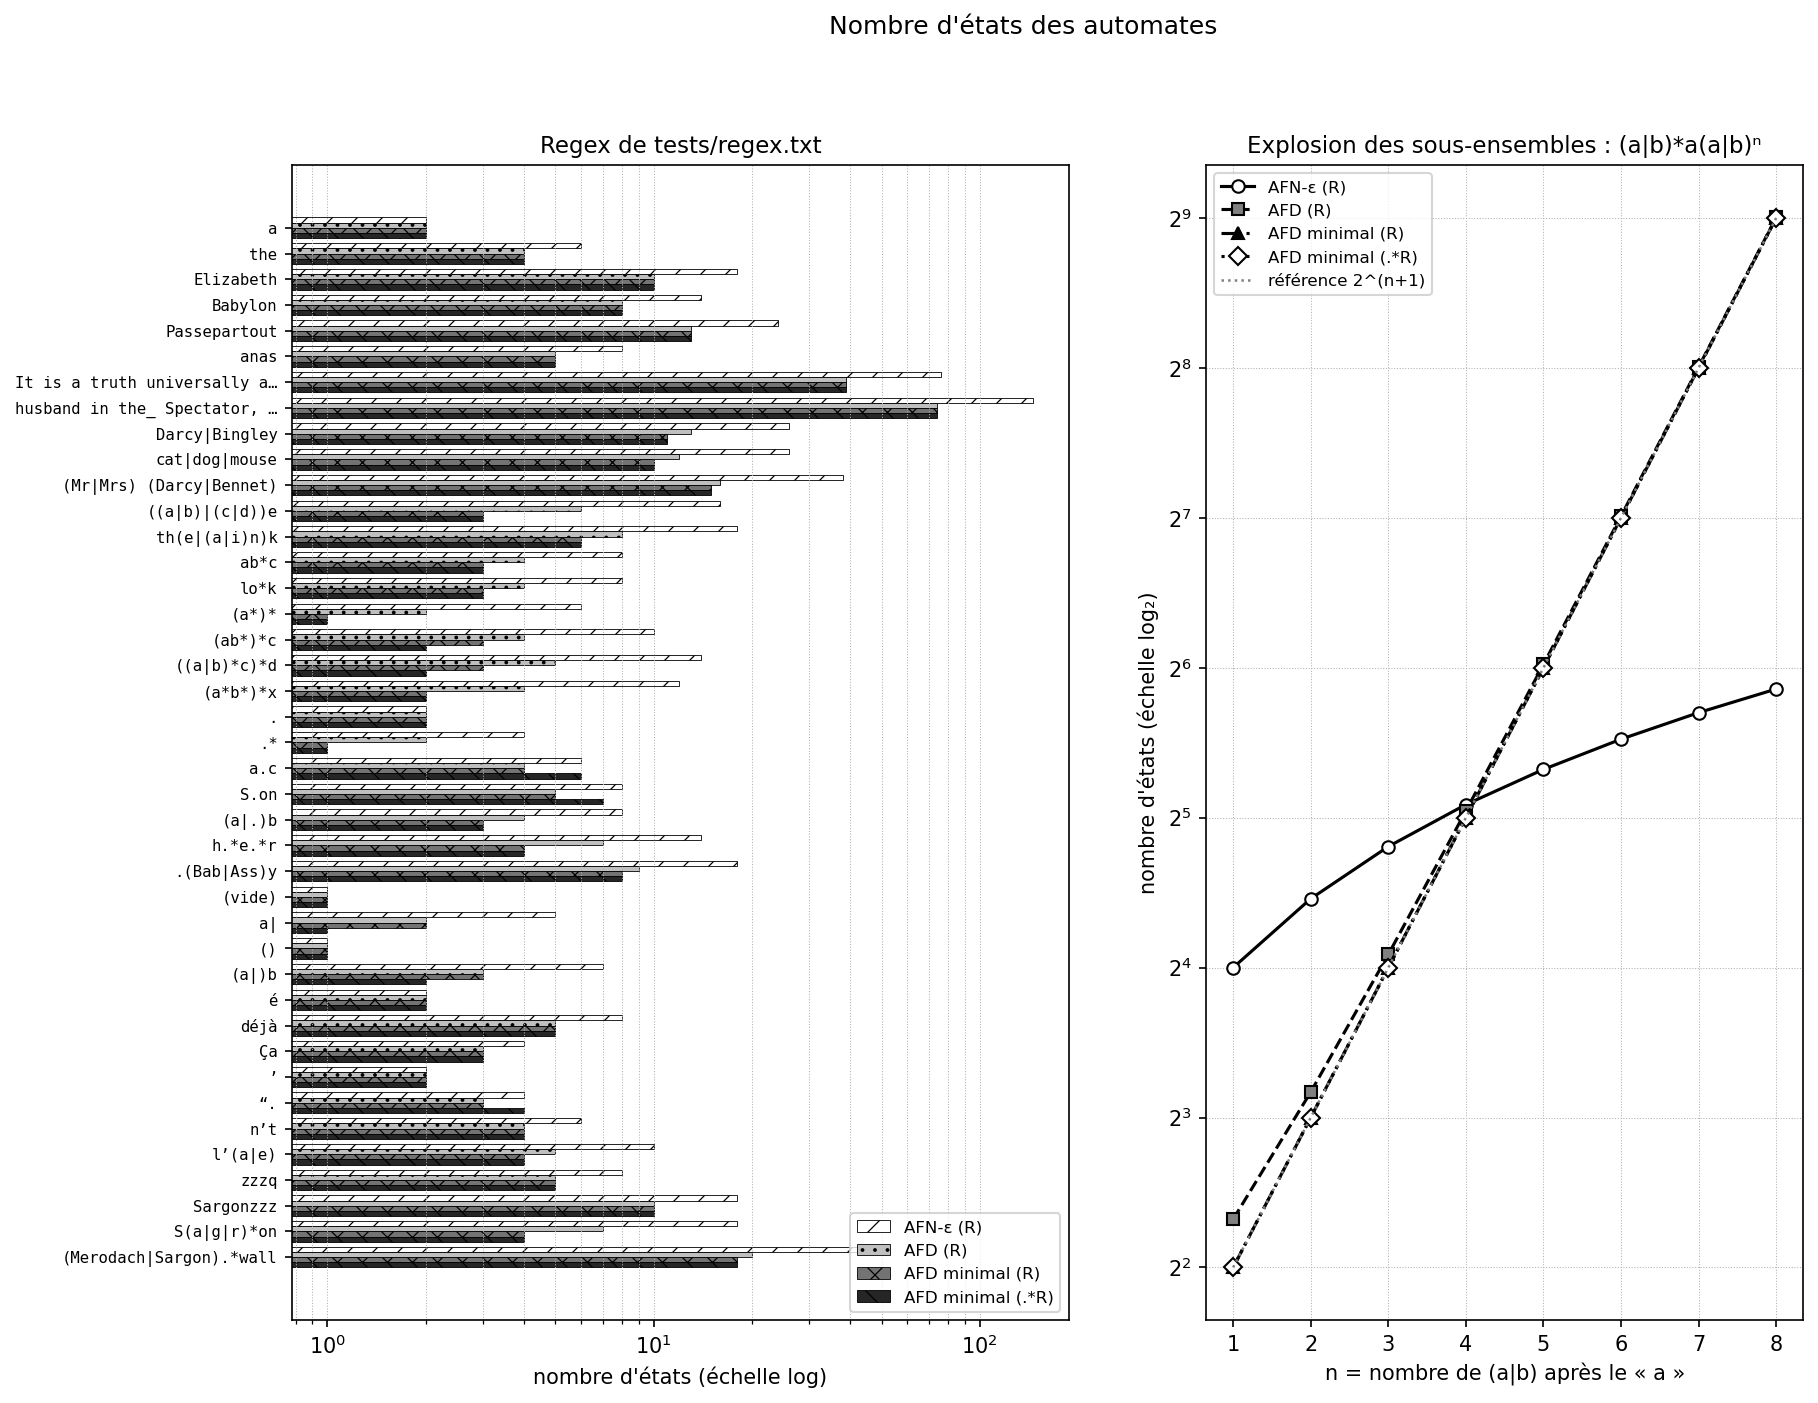
\includegraphics[width=\linewidth]{figures/fig_etats_automates.png}
\end{minipage}\hfill
\begin{minipage}{0.45\linewidth}
\centering
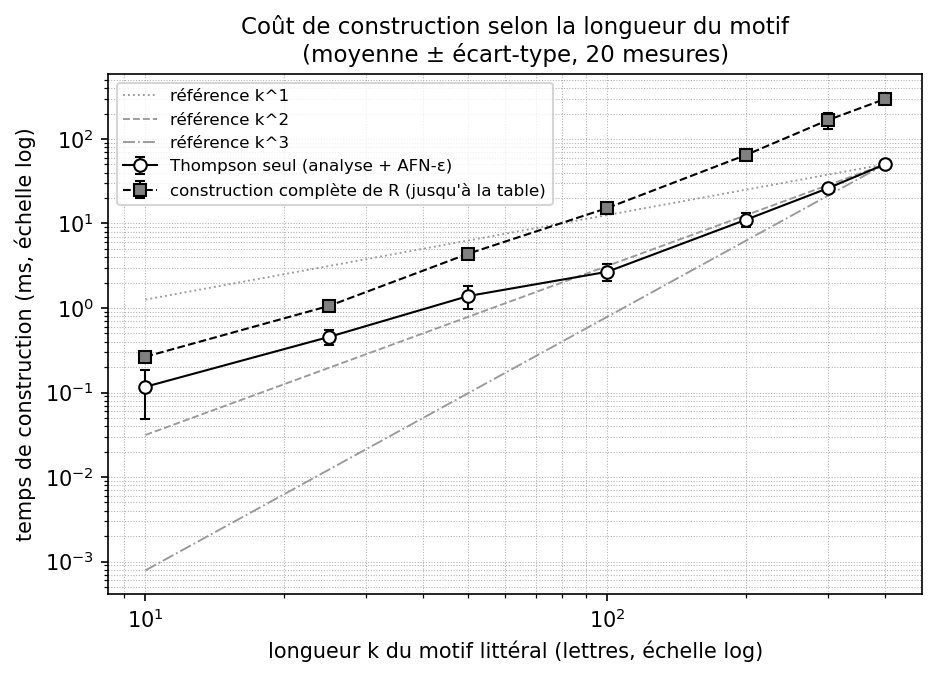
\includegraphics[width=\linewidth]{figures/fig_construction_thompson.png}
\end{minipage}
\caption{À gauche : nombre d'états, sans l'état puits, des automates des
41 regex du banc et de \texttt{(a|b)*a(a|b)}$^n$ (référence $2^{n+1}$). À
droite : temps de construction selon la longueur $k$ d'un littéral.}
\label{fig:monstre}
\end{figure}

\subsection{L'impatient : notre programme contre \texttt{grep}}

On tape une commande et on attend : seul compte le temps total.
\begin{verbatim}
time java -jar egrep-clone.jar -c the data/yellow-wallpaper-1952.txt
\end{verbatim}
La méthode est celle de \texttt{-{}-algo=auto}, mais ici l'algorithme
décide peu. De bout en bout (figure~\ref{fig:bout}), \texttt{grep} est
5 à 75 fois plus rapide que nous. Les deux extrêmes :
\texttt{a.c} sur le fichier de 32~Mio (415,7~$\pm$~21,2~ms contre
80,2~$\pm$~1,5~ms, soit 5,2) et \texttt{S(a|g|r)*on} sur \emph{The Yellow
Wallpaper} (99,7~$\pm$~24,5~ms contre 1,32~$\pm$~0,02~ms, soit 75). Le
démarrage de la JVM pèse lourd : sur un fichier vide, avec \texttt{zzzq},
notre programme met 58,5~$\pm$~5,0~ms et \texttt{grep} 1,4~$\pm$~0,2~ms.
Sur 32~Mio, nos temps varient peu selon la regex, de
334,1~$\pm$~33,2~ms (\texttt{zzzq}) à 421,0~$\pm$~26,5~ms
(\texttt{(Mr|Mrs) (Darcy|Bennet)}).

\begin{figure}[htbp]
\centering
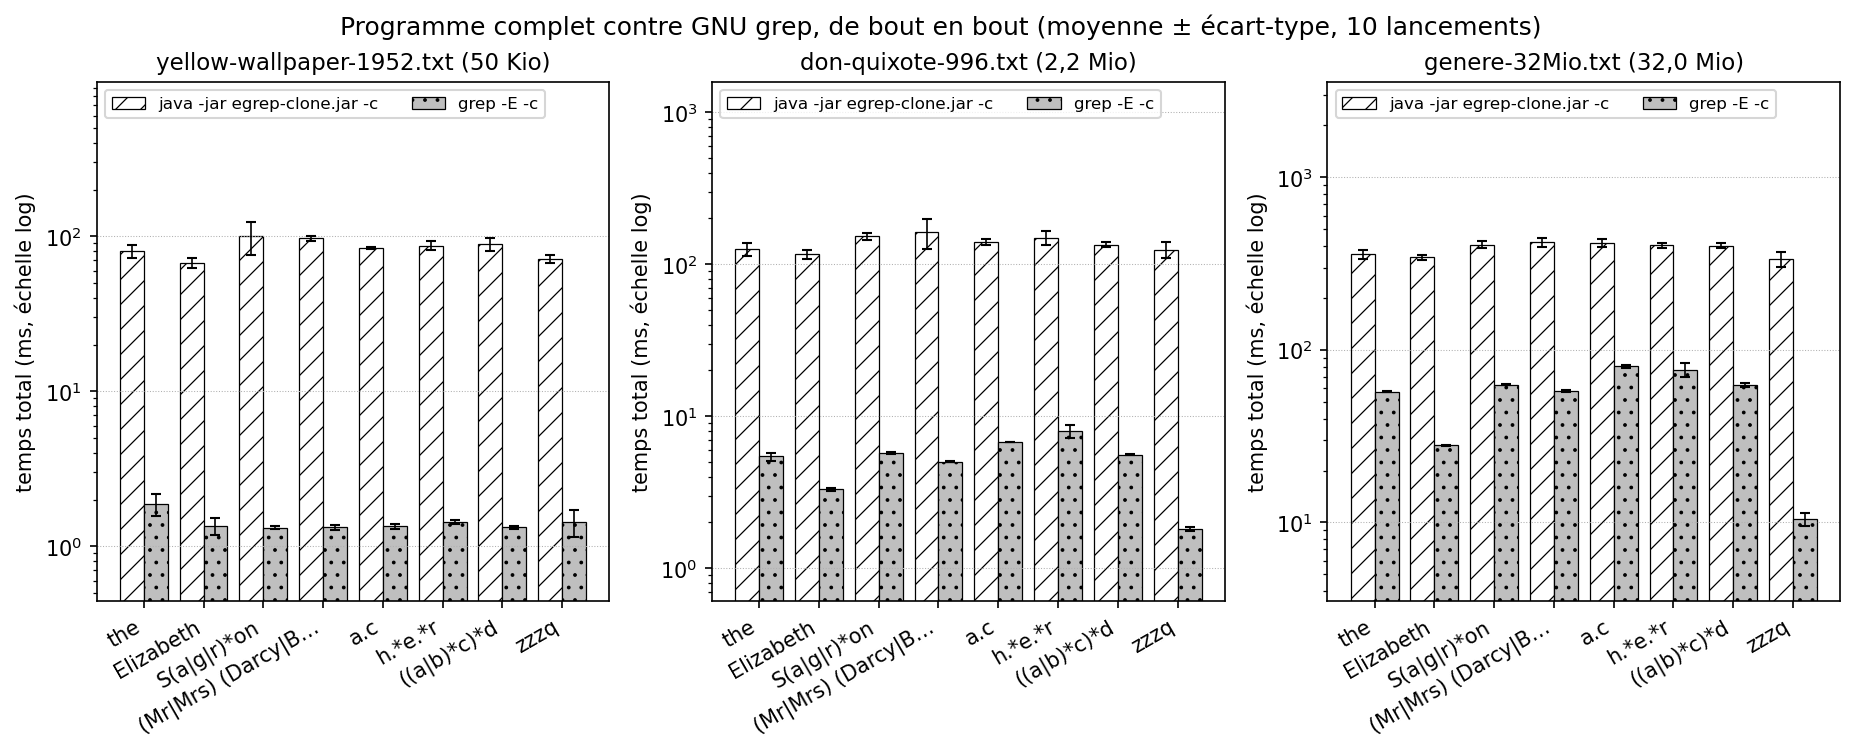
\includegraphics[width=\linewidth]{figures/fig_bout_en_bout.png}
\caption{Programme complet (\texttt{java -jar egrep-clone.jar -c}) contre
\texttt{grep -E -c}, 8 regex sur 3 fichiers, démarrage compris
(10 lancements, échelle log).}
\label{fig:bout}
\end{figure}

%% DISCUSSION À ÉCRIRE ENSEMBLE
